\chapter{無線LANセキュリティ演習}

\section{概要}

無線LAN攻撃演習では,Aircrack-ngを用いて無線LANのWEPキーを解読した.
また,解読したWEPキーを用いて盗聴したパケットを復号し,通信の内容を読み取れることを
確認した.

\section{実験内容}

\subsection{実験環境}

実験には,WEP暗号化に対応した無線LANルータと,無線LANクライアント機能を備えた2台のノートPCを用いた.

\begin{itemize}
\itemsep1pt\parskip0pt\parsep0pt
\item
  無線LANルータ:
  ルータモードで動作させ,13文字のパスワードによるWEP暗号化を設定した.インターネットや他のネットワークには接続せず,独立したネットワークを構築した.
\item
  ノートPC1:
  このPCは,WEPキーの解読に必要なパケットを発生させるために使用した.ノートPC1は,無線LANルータのIPアドレスへpingを送り続けるように設定した.
\item
  ノートPC2:
  このPCで,Aircrack-ngを実行し,実際にWEPキーの解読を行った.
\end{itemize}

\subsection{実験手順(WEPキーの解読)}

\begin{enumerate}
\def\labelenumi{\arabic{enumi}.}
\itemsep1pt\parskip0pt\parsep0pt
\item
  \texttt{airmon-ng}で使用できる無線LANインターフェースカードの一覧を表示した.
\item
  \texttt{airmong-ng}で無線LANインターフェースカードをモニタモードに投入した.
\item
  \texttt{airodump-ng}で通信できる無線LANアクセスポイントの一覧を表示し,解読対象の無線LANルータのBSSIDとチャネルを調べた.
\item
  \texttt{airodump-ng}を3.で調べたBSSIDとチャネルを指定して起動し,パケットのキャプチャした.
\item
  \texttt{airodump-ng}を実行した状態で,\texttt{aircrack-ng}を起動し,解読した.
\end{enumerate}

\subsection{実験手順(通信の盗聴)}

\begin{enumerate}
\def\labelenumi{\arabic{enumi}.}
\itemsep1pt\parskip0pt\parsep0pt
\item
  \texttt{airodump-ng}で対象の無線LANルータのパケットをキャプチャした.
\item
  実験手順(WEPキーの解読)の手順に従いWEPキーを解読した.
\item
  \texttt{airdecap-ng}にキャプチャファイルと解読したWEPキーを与え,キャプチャファイルを復号した.
\item
  復号したキャプチャファイルをWiresharkで開いた.
\end{enumerate}

\section{実験結果}

無線LANルータに設定した13文字のWEPキーは,\texttt{aircrack-ng}を起動してから約5分弱で正しく解読することができた.また,解読したWEPキーを用いてキャプチャしたパケットを解読したところ,HTTP通信などを解読することができた.

\section{考察}

WEP(Wired Equvivalent Privacy)はRC4(Rivest Cipher
4)を暗号化に用いている.RC4は同じ暗号鍵で異なる鍵ストリームを生成するために,IV
(Initialization Vector, 初期化ベクトル)
というものを用いている.この初期化ベクトルは24bitの長さしか持たないため,トラフィック量が多いと,同じ初期化ベクトルが再利用される可能性がある.また,平文のIPヘッダやSNAPヘッダが予測可能である事実も存在する.これらの脆弱性を活用し,統計的なアルゴリズムによりAircrack-ngはWEPキーを短時間で解読することが可能である.

\begin{figure}[htbp]
    \begin{center}
        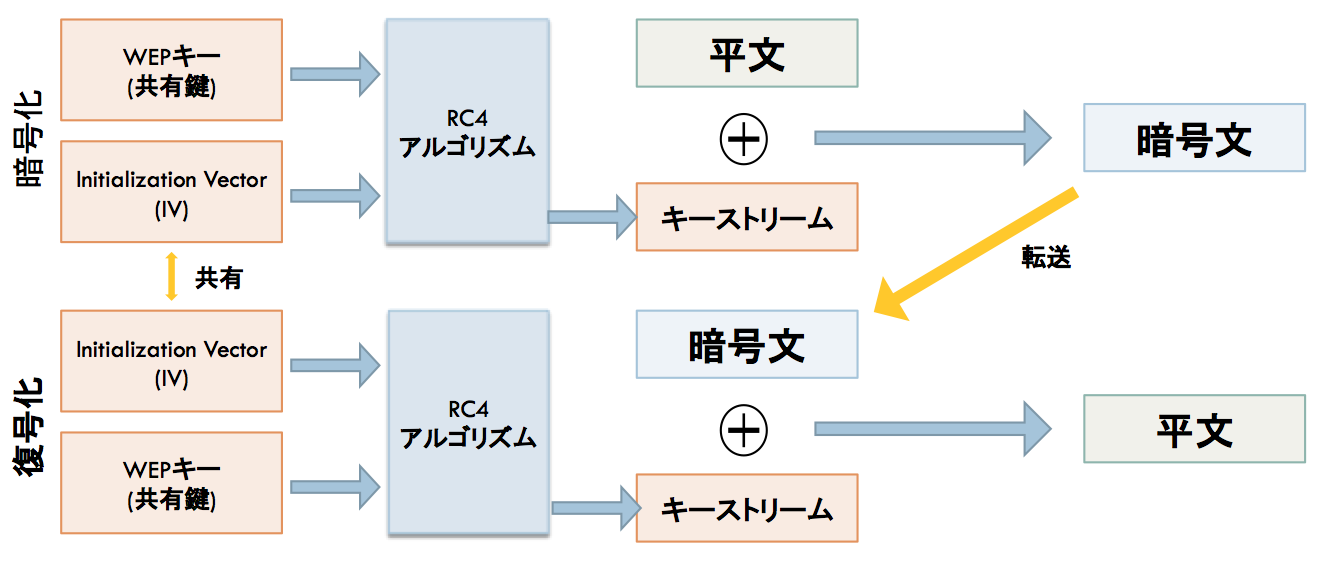
\includegraphics[width=120mm]{wep.png}
    \end{center}
    \caption{WEPの暗号化アルゴリズムの概要}
\end{figure}

今回の実験で確認したように,WEPキーは簡単に解読することが可能であり,セキュリティ上のリスクとなり得る.これを防ぐために,暗号化方式をWEPから,802.11iで定義されているWPA2-PSK
(AES)やWPA2-EAP(AES)
に置き換えることが効果的である.ただし,WPA2も辞書攻撃に対する脆弱性が存在するために,予測不可能で十分に長いパスフレーズを選択することが重要である.しかし,デバイスがレガシーであるなど,諸々の事情によりやむを得ずにWEPを使用しなければいけない状況もある.そのような場合には,TLS
(Transport Layer Security),VPN(Virtual Private Network)
,SSHトンネリングなど,上位層における暗号化によりある程度安全性を確保することが可能である.
